\section{Preliminary Modeling}\label{Sect:modelPrep}

\subsection{Lennard-Jones Potential}\label{Sect:LJPotential}
Before jumping to quantum mechanical data, this math will be tested to construct models on a simplified potential, the Lennard-Jones potential. Though the Lennard-Jones potential is a simplification of reality, it does a excellent job representing real intermolecular forces of attraction and repulsion. The potential is a function of distance between two particles given by

\begin{equation} \label{LJ}
V_{LJ}(r) = 4\varepsilon \bigg[\Big(\frac{\sigma}{r}\Big)^{12} - \Big(\frac{\sigma}{r}\Big)^6\bigg],
\end{equation}
where $\varepsilon$ and $\sigma$ are constants for a given particle interaction. Figure \ref{figLJ} shows the plot of this potential.

\begin{figure}[h]
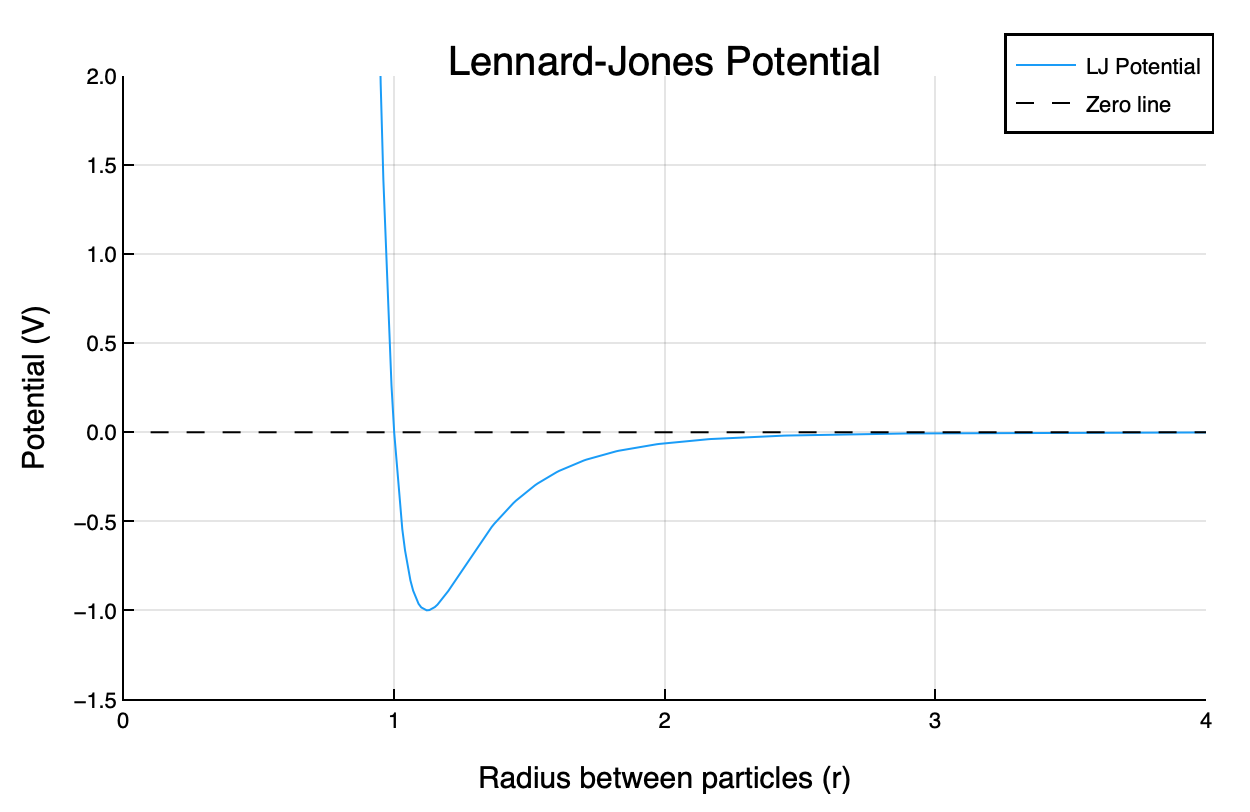
\includegraphics[scale = 0.4]{Figures/LJPotential}
\caption{The Lennard-Jones potential. A simple yet realistic model of intramolecular forces.
\label{figLJ}} 
\end{figure}

\par It can be recalled that the force from a potential is given by

\begin{equation} \label{forceEq}
F = -\nabla U,
\end{equation}
and thus the force between two particles is zero at the bottom of the potential well. With that location as a reference, distances any greater will produce a force that is attractive and at any lesser distances, the force is intensely repulsive.
\par Calculating the potential between two particles is not difficult, but finding the total potential energy of a system of several particles becomes increasingly computationaly expensive. Because of the simplicity of the Lennard-Jones potential, the computational power required to solve for the system's energy is still relatively small. In preparation for using real, quantum-mechanical data, each system's energy will be treated as expensive to compute. 



\subsection{Constructing a Model}\label{Sect:LJModels}
\par Ensuring a sufficient number and breadth of samples as well as reasonable basis functions becomes difficult as the number of dimensions goes beyond 2 or 3. From studying a variety of potential basis functions, bessel functions of the second kind, $Y_\alpha(x)$, have the potential to be useful.
\par Rewriting Equation \ref{fundLinAlg} in component form yields


\begin{equation}
\begin{bmatrix}
A_{11} & A_{12} & \ldots & A_{1m} \\
A_{21} \\
\vdots & & & \vdots\\
A_{n1} & \ldots & & A_{nm}
\end{bmatrix}
\begin{bmatrix}
b_0 \\
b_1 \\
b_2 \\
\vdots \\
b_m 
\end{bmatrix}
=
\begin{bmatrix}
V_1 \\
V_2 \\
V_3 \\ 
\vdots \\
V_n
\end{bmatrix}.
\label{AMatrix}
\end{equation}

\par Recognizing each row of $A$ as a unique sample, Equation \ref{AMatrix} can be written as a system of linear equations

\begin{align}
A_{11}b_1 + A_{12}b_2 + A_{13}b_3 + ... + A_{1n}b_n &= V_1 \\
A_{21}b_1 + A_{22}b_2 + A_{23}b_3 + ... + A_{2n}b_n &= V_2.
\end{align}

\par Each element of $A$ will be populated with
\begin{align}
A_{11} &= Y_0(\alpha_{01} r_{12}) + Y_0(\alpha_{01} r_{13}) + Y_0(\alpha_{01} r_{23}) + \ldots \\
A_{12} &= Y_0(\alpha_{02} r_{12}) + Y_0(\alpha_{02} r_{13}) + Y_0(\alpha_{02} r_{23}) + \ldots  \\
A_{1n} &= Y_0(\alpha_{0n} r_{12}) + Y_0(\alpha_{0n} r_{13}) + Y_0(\alpha_{0n} r_{23}) + \ldots
\end{align}
where $\alpha_{0n}$ is the $n$-th zero of $J_0$, the zeroth bessel function of the first kind.

\begin{figure}[h]
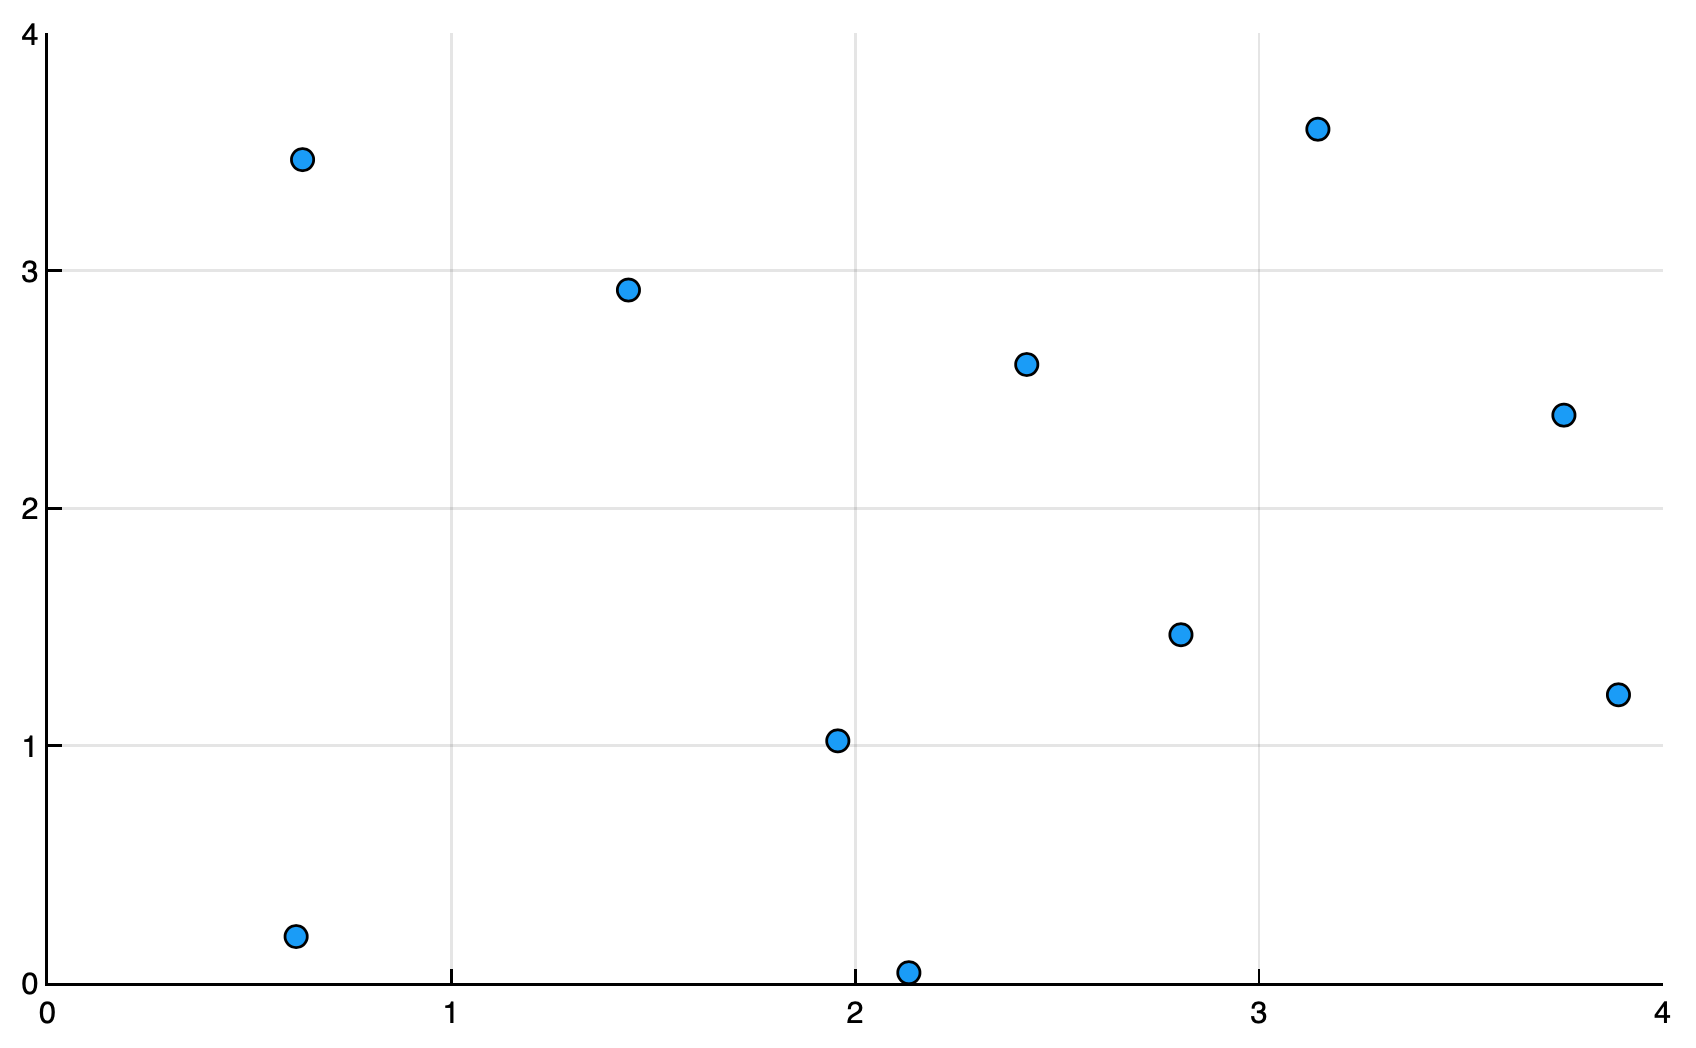
\includegraphics[scale = 0.3]{Figures/tenParticles}
\caption{A random assortment of 10 particles in a 4x4 square. No two particles are allowed to be within a pre-specified distance of each other. 
\label{tenParticles}} 
\end{figure}

\begin{itemize}
\item Minimum separation distance
\item Number of particles in box
\item Sample/function num
\item Why separation vector norms?
\item 
\end{itemize}




\subsection{Multi-Type Particle Systems}\label{Sect:diatomic}
\par Now that a simple monotomic model has been constructed, it can be adjusted to handle two different types of particles. The different particles can be labeled type-$A$ and type-$B$. This diatomic system will now require \textit{three} different potential equations, one describing each type of interaction. The three unique interactions are type-$A$ interacting with another type-$A$, a type-$A$ interacting wtih a type-$B$, and a type-$B$ with another type-$B$. Because these are arbitrary interactions, they can be defined by choosing reasonable values of $\varepsilon$ and $\sigma$ from Equation \ref{LJ}. 

\begin{align}
V_{AB}(r) &= 4 \bigg[\Big(\frac{1}{r}\Big)^{12} - \Big(\frac{1}{r}\Big)^6\bigg] \label{LJ} \\
V_{AA}(r) &= 4 (0.7) \bigg[\Big(\frac{0.8}{r}\Big)^{12} - \Big(\frac{0.8}{r}\Big)^6\bigg] \label{LJ} \\
V_{BB}(r) &= 4 (0.4) \bigg[\Big(\frac{1.1}{r}\Big)^{12} - \Big(\frac{1.1}{r}\Big)^6\bigg] \label{LJ}
\end{align}
The graph of each potential can be seen in Figure \ref{fig3LJ}. Each of the equilibrium positions and energies is slightly different, but all in the same neighborhood.

\begin{figure}[h]
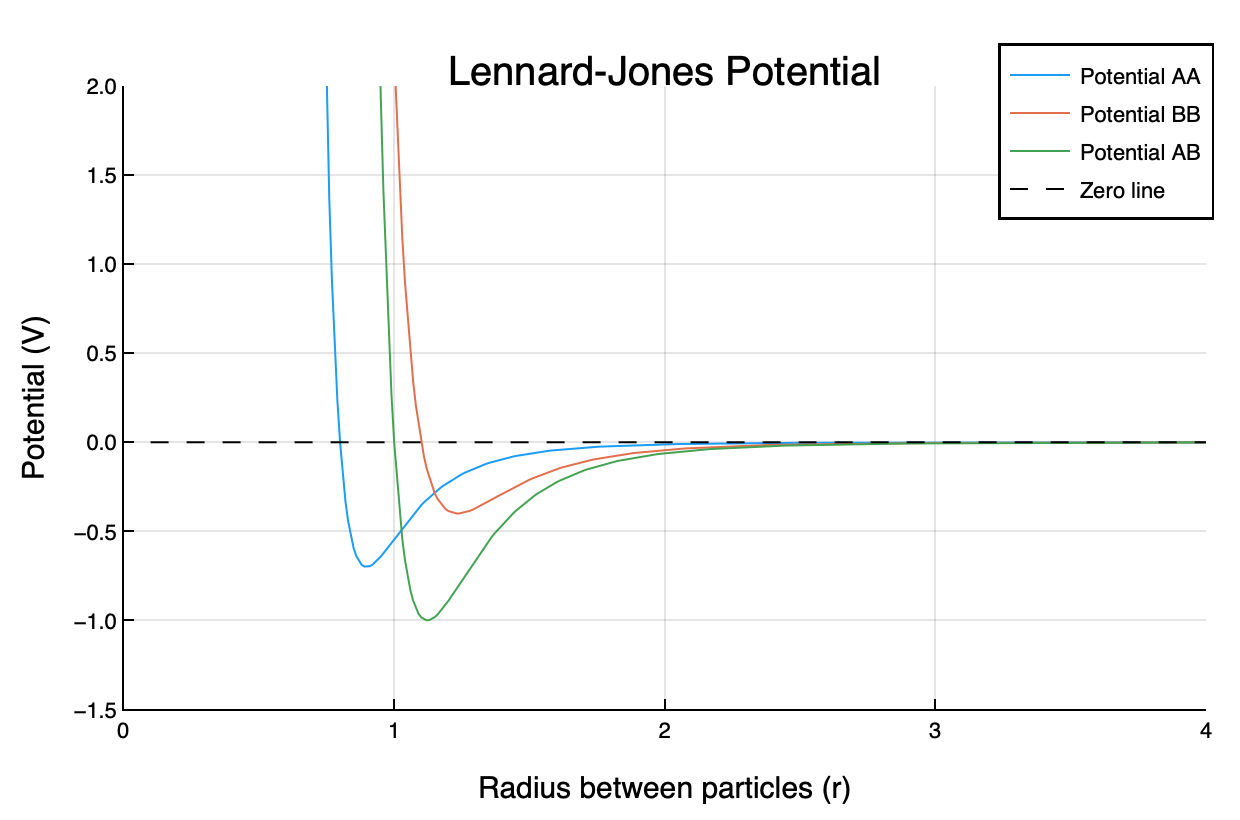
\includegraphics[scale = 0.4]{Figures/newLJPotential}
\caption{A Lennard-Jones potential for each particle interaction type (AA, AB, and BB). Each interaction potential has a slightly different equilibrium position and energy. 
\label{fig3LJ}} 
\end{figure}

\par To handle this increase in complexity, matrix $A$ will need to contain \textit{three} columns where the previous model had only one. This is again because of the three different interaction types, one column for each. Another obstacle arises in the decision for particle type ratio. If the particle number (10) and box size ($4\times4$) remain constant, how many type-$A$ versus type-$B$ particles should there be? The question is really just a general question specified to this case; what is a sufficient breadth of samples for this model? As previously discussed, this depends greatly upon the desired range of predictions. As will be seen in Chapter \ref{procedureData}, the configurations vary in particle number as well as ratio. Therefore, this model should be trained and tested using a variety of particle ratios. Each training and testing set will thus be given a random number and ratio of particles to be populated in and calculated. 
\par Once a model has been properly constructed and trained, how can its accuracy be easily determined and visualized?


\begin{itemize}
\item Particle type ratio
\item Show model accuracy
\end{itemize}



